\section{Aufbau des Systems}
\subsection{Systembeschreibung}
% Bild für Systembeschreibung
\begin{figure}[H]
\centering 
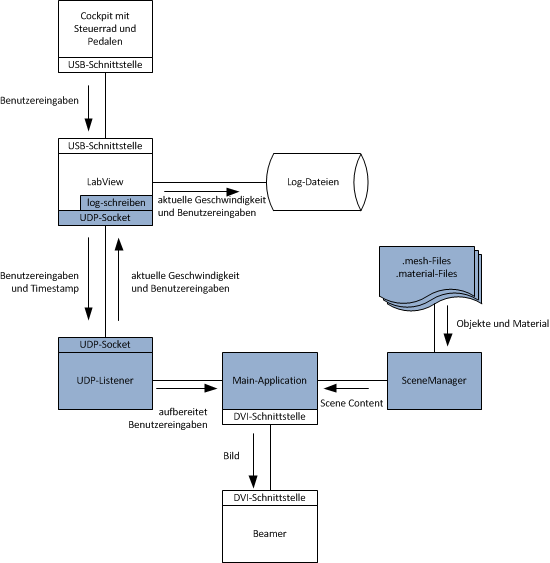
\includegraphics{src/Systembeschreibung.png}
\caption{Systembeschreibung} % Titel der Grafik
\label{Systembeschreibung} % Labelname
\end{figure}

Der Aufbau des Systems für den Fahrsimulator wird anhand der Abbildung \ref{Systembeschreibung} ilustriert. Die blau markierten Komponenten werden im Rahmen dieser Projekt Arbeit entwickelt. Alle übrigen sind bereits vorbestehend. 
Benutzereingaben, die im Cockpit gemacht werden, werden von einem LabView Programm eingelesen. Nun benötigt es einen UDP-Port,  über den verschiedenen Eingaben an das Programm weitergeleitet werden. Es handelt sich hierbei um Werte, die das Drehen des Steuerrades und den Druck auf Gas- oder Bremspedal quantifizieren. Zusätzlich wird der UDP-Port auch für das Empfangen diverser Log-Daten, die von unserem Programm gesendet werden, verwendet. Damit die Empfangenen Daten sauber in ein Log-File geschrieben werden, wird das LabVIEW Programm erweitert. 
Weiter  muss in Programmiersprache C einen UDP-Socket mit entsprechendem UDP-Listener implementieren werden, um die Benutzereingaben zu empfangen. Gleichzeitig wird der UDP-Listener dazu verwendet die Geschwindigkeit des Fahrzeugs sowie Timestamps und weitere Daten an das LabVIEW Programm zurück zu schicken. Damit können die Daten gespeichert und später ausgewertet werden.
\\
Diese Aufteilung durch eine Netzwerkschnittstelle ermöglicht es,  das System, wenn notwendig, zu dezentralisieren. Einfahheitshalber wurde der UDP-Listener erst in einem Video-Beispiel implementier und getestet (Siehe Anhang B). Nachfolgend wird dieser UDP-Listener auch in das Programm des Fahrsimulator transferiert.
Sind die Daten vom UDP-Listener empfangen und aufbereitet, werden sie im Hauptprogramm (Main Application) weiter verwendet. Während die Position des Steuerrades, des Gas und Bremspedales vom UDP-Listener permanent an das Hauptprogramm übertragen werden, wertet dieses die Positionen aus und veranlass die entspechenden Aktionen in der geladenen Szene. 
Die Szene selbst wird von einem Szenen-Manager geladen. Dieser benötig für die zu ladenden Objekte ein Meshfiles und mindestens ein Materialfile. Die Form jedes Objektes in der Szene wird durch ein separates Meshfile definiert. Texturen und Materialien werden durch ein oder mehrere Materialfiles beschrieben. Ein Materialfile kann zur Beschreibung unterschiedlicher Objekte verwendet werden. Die berechnete Szene wird schlussendlich in einem Fenster von Hauptprogramm angezeigt und über eine DVI-Schnittstelle an den Beamer übertragen. Der Beamer projeziert das Bild an die Wand, die sich direkt vor dem Cockpit befindet. 

\subsection{Anforderungen}
\subsubsection{Funktionale Anforderungen}
\begin{itemize}
\item Der Proband kann das Fahrzeug im Fahrsimulator durch manipulation am Steuerrad und der Pedalen im Cockpit steuern.
\item Die aktuelle Geschwindigkeit der Fahzeuges wird dem Probanden angezeigt.
\item Es sollen zwei unterschiedliche Szenen zur verfügung gestellt werden.  Die eine Szene sollte eine Stadt darstellen und die andere Szene eine Landschaft mit Tunnels.
\item Die manipulationen des Benutzers und wichtige Parameter wie z.B. Geschwindigkeit sollen in einer Datei aufgezeichnet werden um diese auszuwerten.
\item Alle ein- und ausgehenden Parameter des System sollen in LabVIEW verfügbar sein um diese auswerten und kontrollieren zu können. 
\end{itemize}
\subsubsection {Nicht Funktionale Anforderungen}
\renewcommand{\labelenumi}{\alph{enumi})}
\begin{enumerate}
\item Zuverlässigkeit\\
Das System soll robust sein. 
\item Benutzbarkeit\\
Das Starten des Fahrsimulator sollte möglichst einfach gehalten werden. Das Steuer des Fahrzeuges soll möglichst intuitiev sein wie man es sich von einem richtigen Fahrzeug gewöhnt ist. 
\item Aussehen und Handhabung\\
Der Fahrsimulator soll dem Probanden eine möglichst realistische Fahrsimulation bieten in der sich Strassen und verschiedene Objekte befinden.
\item Zeitliche Anforderungen\\
Die Raktionszeit des Systems soll möglichst klein sein. Die Verzögerung des Systems soll mess-  und kalkulierbar sein.
\item Erweiterbarkeit\\
Das System soll möglichst Modular aufgebaut sein um später einfach erweitert werden zu können.
\item Portierbarkeit\\
Das System soll auf der existierender Hardware funktionieren, soll aber auch noch lauffähig sein wenn Teile des Fahrsimulators ausgetauscht werden. 
\end{enumerate}
